\documentclass[11pt]{article}
\usepackage[utf8]{inputenc}
\usepackage[T1]{fontenc}
\usepackage[margin=1in]{geometry}
\usepackage{graphicx}
\usepackage{enumitem}
\usepackage{parskip}
\usepackage{tabularx}
\usepackage{array}
\usepackage{hyperref}
\usepackage{titlesec}

\titleformat{\section}{\Large\bfseries}{}{0pt}{}
\titleformat{\subsection}{\large\bfseries}{}{0pt}{}
\titleformat{\subsubsection}{\normalsize\bfseries}{}{0pt}{}

\setlist[itemize]{leftmargin=*,itemsep=2pt,parsep=0pt}

\begin{document}

\begin{titlepage}
\centering
\vspace*{\fill}

{\Huge\bfseries Bubble Buddies\par}
\vspace{0.35cm}
{\Large\itshape Bubble Sort in LC-3 Assembly\par}

\vspace{1.2cm}

{\Large CIS 11 \textemdash{} Course Project\par}
\vspace{0.2cm}
{\large Project Documentation\par}

\vspace{1.2cm}

{\large Samuel Gerungan\par}
\vspace{0.1cm}
{\large Tyla Robertson\par}

\vspace{1.2cm}

{\normalsize Advisor: Kasey Nguyen, PhD\par}
\vspace{0.25cm}
{\normalsize May 24, 2026\par}

\vspace*{\fill}
\end{titlepage}

\section*{Part I -- Application Overview}

\subsection*{Objectives}

Bubble Buddies is our team's bubble sort program written in LC-3 assembly. The goals for the project are listed below.


\subsubsection*{Project objectives}

\begin{itemize}
  \item Learn to use LC-3 assembly: registers, the instruction set, assembler directives, and the TRAP system calls.
  \item Use the main parts of assembly in one program: arithmetic and data-movement instructions, conditional and iterative branching, subroutine calls, pointers, and ASCII conversion for keyboard input and console output.
  \item Write a working bubble sort in LC-3 assembly that we can test with the required input.
  \item Work as a team: split the work between us, agree on coding conventions, and share the documentation.
\end{itemize}
\subsubsection*{Motivation}

This is the final project for the assembly programming unit in CIS 11. It puts together most of what we covered in the course: registers, the instruction set, subroutines, the stack, and ASCII input and output.


\subsubsection*{Who the project is for}

\begin{itemize}
  \item Our team (Samuel Gerungan and Tyla Robertson). The project gives us one program where we use everything from the assembly unit.
  \item The instructor (Kasey Nguyen, PhD). She has something to grade and to check what we learned.
  \item Future students. The documented program can be used as an example of bubble sort in LC-3.
\end{itemize}

\subsection*{Business Process}

The program runs by itself in an LC-3 simulator. It does not connect to any other software, and it is not replacing anything.


\subsubsection*{How a user runs the program}

\begin{itemize}
  \item 1. The user launches an LC-3 simulator and loads the assembled object file at origination address x3000.
  \item 2. The user initiates program execution.
  \item 3. The program displays an on-screen prompt requesting eight numbers, each in the range 0-100.
  \item 4. The user enters the eight numbers one at a time, terminating each entry with the Enter key.
  \item 5. The program reads each entry as ASCII characters, converts the value to its integer equivalent, and stores it in a fixed-size in-memory array.
  \item 6. Once all eight values are stored, the program sorts the array into ascending order by repeated pairwise comparison and swap.
  \item 7. The program converts each sorted integer back to ASCII and displays the eight values, in ascending order, on the console.
  \item 8. The program halts cleanly via the HALT trap.
\end{itemize}

\subsection*{User Roles and Responsibilities}

There is one user role (the person running the program) and two project roles (the developers and the instructor).


\subsubsection*{User (the person running the program)}

\begin{itemize}
  \item What they do: start the simulator, load the program, type in eight numbers, look at the sorted output, close the simulator.
  \item How often: once per run. The program is short and can be run again easily.
  \item Input: eight whole numbers between 0 and 100, typed in as digits.
  \item Output: the prompt asking for numbers, and the sorted list printed to the console.
\end{itemize}
\subsubsection*{Developers (Samuel Gerungan and Tyla Robertson)}

\begin{itemize}
  \item What we do: design the program (objectives, pseudocode, flowchart), write the LC-3 code, assemble and test it, fix bugs, write comments and documentation, and submit the project.
  \item Submission: each of us submits the documentation; the source code is shared through our team git repository.
  \item How we have split the work so far: Samuel is writing the project documentation, and Tyla is writing the pseudocode and drawing the flowchart. The LC-3 source code in Part 3 will be split between us, with details recorded in the Team Sign Up document.
\end{itemize}
\subsubsection*{Instructor (Kasey Nguyen, PhD)}

\begin{itemize}
  \item What she does: reads the documentation, grades the program, and gives us feedback we can use to revise.
\end{itemize}

\subsection*{Production Rollout Considerations}

The project is turned in across three parts, following the course schedule. There is no earlier version of the program that we need to switch users away from.


\subsubsection*{Project parts}

\begin{itemize}
  \item Part 1 -- Documentation. Submit this project documentation and the Team Sign Up document. Each team member uploads the documentation on their own.
  \item Part 2 -- Details to be confirmed with the instructor.
  \item Part 3 -- Build and test. Submit the LC-3 source code, assembled and tested, along with the result of the acceptance test described in the Scope section.
\end{itemize}
\subsubsection*{Data and run size}

The program handles eight 16-bit numbers per run and works as fast as the user can type. Nothing is saved between runs. The program fits easily in the LC-3 user memory starting at x3000.


\subsection*{Terminology}

Short definitions for the technical terms used in this document.


\begin{itemize}
  \item LC-3 -- 'Little Computer 3', the 16-bit instruction-set architecture used as the teaching platform in CIS 11. Eight general-purpose registers (R0-R7), 16-bit memory addressing, a small instruction set, and the assembler directives .ORIG, .FILL, .BLKW, .STRINGZ, .END.
  \item Bubble sort -- a comparison-based sorting algorithm in which each pair of adjacent elements is compared and swapped if out of order, the pass repeating until no swaps occur. Worst-case and average time complexity O(n\textasciicircum{}2).
  \item Origination address -- the starting memory address at which the program is loaded and begins execution, specified via .ORIG. The program uses x3000, the conventional LC-3 user-program origin.
  \item Subroutine -- a callable block of code, invoked with JSR (which writes the return address into R7) and returned from with RET (which jumps to the address in R7).
  \item Stack -- a region of memory used for saving registers between subroutine calls. The LC-3 does not have a built-in stack, so the program manages one in software.
  \item PUSH / POP -- the two stack operations. PUSH writes a register value onto the stack; POP reads it back off.
  \item Save / restore -- saving a subroutine's working registers at the start (with PUSH) and restoring them before returning (with POP), so the main program's registers are not changed by the call.
  \item Pointer -- a register that holds the address of a memory location, used with LDR / STR (base + offset) for indirect access and array traversal.
  \item TRAP -- the LC-3 system-call mechanism. The trap vector selects a service routine: x20 GETC, x21 OUT, x22 PUTS, x25 HALT.
  \item ASCII -- character encoding used for console input and output. The digit characters '0'-'9' occupy code points x30-x39; integer-to-ASCII conversion is performed by adding x30, and ASCII-to-integer by subtracting it.
  \item Overflow -- a value that goes outside the allowed range, either because a number is too large to store or because the program tries to write past the end of the array.
  \item READNUM -- the subroutine responsible for reading one decimal number from the keyboard. Returns the parsed integer.
  \item PRINTNUM -- the subroutine responsible for printing one decimal number to the console. Emits each digit as an ASCII character.
\end{itemize}

\section*{Part II -- Functional Requirements}

\subsection*{Statement of Functionality}

The program performs the steps listed below, in order. It uses two subroutines, READNUM and PRINTNUM; the input loop, the sort, and the output loop run in the main program.


\begin{itemize}
  \item Start the program at memory address x3000 (set with .ORIG x3000). Point R6 at the start of ARRAY and set the input counter R5 to 0.
  \item Print the prompt "Enter 8 numbers (0-100), ENTER after each:" with PUTS.
  \item Read eight numbers. For each one, call READNUM, store the value into ARRAY through R6, then advance R6 and increment R5.
  \item Hold the inputs in an 8-word array set aside with .BLKW 8.
  \item Sort the array in ascending order with bubble sort. For each pass, walk R6 along the array, load adjacent pairs into R1 and R2, subtract to compare, and swap when the first value is larger.
  \item Print the header "\textbackslash{}nSorted numbers:" with PUTS.
  \item Print the sorted values. Reset R6 to the start of ARRAY, then for each element load it into R0, call PRINTNUM, and print a single space.
  \item Halt with TRAP x25.
\end{itemize}
\subsubsection*{Subroutines}

Each subroutine saves the registers it changes (together with the return address R7) at the start, and restores them before returning, so the main program's registers are not disturbed.


\begin{itemize}
  \item READNUM reads characters from the keyboard with GETC, echoes each one with OUT, and builds up the value digit by digit until ENTER is pressed. The completed number is returned in R0.
  \item PRINTNUM takes a number in R0 and breaks it into hundreds, tens, and ones by repeated subtraction, then prints each digit as a character with OUT.
\end{itemize}
\subsubsection*{Register use}

\begin{itemize}
  \item R0 -- value passed to and from subroutines and TRAPs.
  \item R1, R2 -- adjacent values being compared in the sort.
  \item R3 -- result of the comparison.
  \item R4 -- outer sort-loop counter.
  \item R5 -- counter for the input, sort, and output loops.
  \item R6 -- pointer that walks through ARRAY.
  \item R7 -- return address used by JSR and RET.
\end{itemize}
\subsubsection*{What the program does not do}

The program handles eight numbers at a time and sorts them with bubble sort. Larger inputs, other sort algorithms, and saving results between runs are not part of this project.


\subsection*{Scope}

The project is delivered in three parts. Below is what each part includes, plus what we are not building.


\subsubsection*{What is in each part}

\begin{itemize}
  \item Part 1 -- This project documentation and the Team Sign Up document.
  \item Part 2 -- Details to be confirmed with the instructor.
  \item Part 3 -- The LC-3 source code, assembled and tested, running every step in the Statement of Functionality and passing the acceptance test below.
\end{itemize}
\subsubsection*{Acceptance test}

The program passes when, given the inputs 11, 8, 2, 17, 6, 4, 3, 21, it prints 2, 3, 4, 6, 8, 11, 17, 21 to the console and halts.


\subsubsection*{What we are not building}

Sorting more than eight numbers, any sort other than bubble sort, file input or output, a graphical interface, and input checking beyond the overflow handling described in the Terminology section.


\subsection*{Performance}

The program is small (eight numbers, fixed-size loops), so it runs fast on any LC-3 simulator. The targets we are aiming for are listed below.


\begin{itemize}
  \item Execution time -- under one second from program start to HALT, not counting the time the user spends typing.
  \item Memory footprint -- under 256 words of LC-3 memory for the program and its data combined.
  \item Response time -- under 100 milliseconds from the user's last keystroke to the first character of sorted output.
\end{itemize}

\subsection*{Usability}

The program is a simple text-mode program that runs in the console. The points below are what we want the experience to be.


\begin{itemize}
  \item Clear prompt -- before asking for input, the program prints a line that says how many numbers to enter (eight), the allowed range (0 to 100), and that each number should be followed by Enter.
  \item Echoed input -- each character the user types appears on the screen as they type it.
  \item Clear output -- the sorted numbers are printed in ascending order on one line, separated by single spaces, under the header "Sorted numbers:" so the output is easy to find.
  \item No interruptions -- once the eight numbers are entered, the program finishes on its own and halts.
\end{itemize}

\section*{Documenting Requests for Enhancements}

No enhancement requests have been received yet. Any future requests will be added to the table below, with the date, a short description, who requested it, the priority, and how it was handled.


\begin{center}
\small
\begin{tabularx}{\textwidth}{|X|X|X|X|X|X|}
\hline
\textbf{Date} & \textbf{Enhancement} & \textbf{Requested by} & \textbf{Notes} & \textbf{Priority} & \textbf{Release No/Status} \\
\hline
 & & & & & \\[1.5em]
\hline
 & & & & & \\[1.5em]
\hline
 & & & & & \\[1.5em]
\hline
\end{tabularx}
\end{center}


\section*{Part III -- Appendices}

The appendices have extra reference material: a short bubble sort review and the list of LC-3 instructions used in the program. The full pseudocode and the flowchart are in the next section.


\subsubsection*{Appendix A -- Bubble sort review}

Bubble sort goes through the array and compares each adjacent pair, swapping them if they are out of order. After each pass, the largest unsorted value ends up at the back. The worst-case and average time complexity is O(n\textasciicircum{}2), and the sort is done in place so it only uses O(1) extra memory.


\subsubsection*{Appendix B -- LC-3 instructions used}

ADD, AND, and NOT for arithmetic and logic; LD, LDI, LDR, and LEA for loading values from memory; ST, STI, and STR for storing them; BR (with the n, z, p condition codes) for branching; JSR and RET for calling and returning from subroutines; and TRAP for the GETC, OUT, PUTS, and HALT system calls. PUSH and POP are written as short sequences of these instructions.


\subsection*{Flow chart or pseudo-code}

\subsubsection*{Pseudocode (high-level, language-agnostic)}

\begin{verbatim}
PROGRAM BubbleBuddies
    .ORIG x3000

    PRINT "Enter 8 numbers (0-100), ENTER after each:"
    CREATE array[8]

    ; Input 8 numbers
    FOR i FROM 0 TO 7:
        array[i] = READNUM()

    ; Bubble sort (ascending order)
    FOR i FROM 0 TO 6:
        FOR j FROM 0 TO 6:
            IF array[j] > array[j + 1]:
                SWAP array[j] AND array[j + 1]

    ; Print sorted array
    PRINT "\nSorted numbers:"
    FOR i FROM 0 TO 7:
        PRINTNUM(array[i])
        PRINT " "

    HALT

SUBROUTINE READNUM():
    number = 0
    LOOP:
        char = GET character from keyboard
        PRINT char                       ; echo it
        IF char IS ENTER:
            BREAK
        digit = char - '0'               ; convert ASCII to number
        number = (number * 10) + digit
    PRINT newline
    RETURN number

SUBROUTINE PRINTNUM(number):
    hundreds = 0
    tens = 0

    ; Count hundreds
    WHILE number >= 100:
        hundreds = hundreds + 1
        number   = number - 100

    ; Count tens
    WHILE number >= 10:
        tens   = tens + 1
        number = number - 10

    ones = number

    ; Print hundreds (if any)
    IF hundreds > 0:
        PRINT (hundreds + '0')

    ; Print tens
    IF tens > 0:
        PRINT (tens + '0')
    ELSE IF hundreds > 0:
        ; special case like 100 -> prints 0 in tens place
        PRINT '0'

    ; Print ones
    PRINT (ones + '0')
\end{verbatim}

\subsubsection*{Flowchart}

The program flowchart is shown below. The diagram covers the input loop (eight READNUM invocations), the inlined bubble-sort phase (outer loop on i, inner loop on j, with the swap conditional), the output loop (eight PRINTNUM invocations with single-space separators), and the internal save/restore discipline of READNUM. Each block is annotated with the LC-3 register operation it performs.

\begin{center}
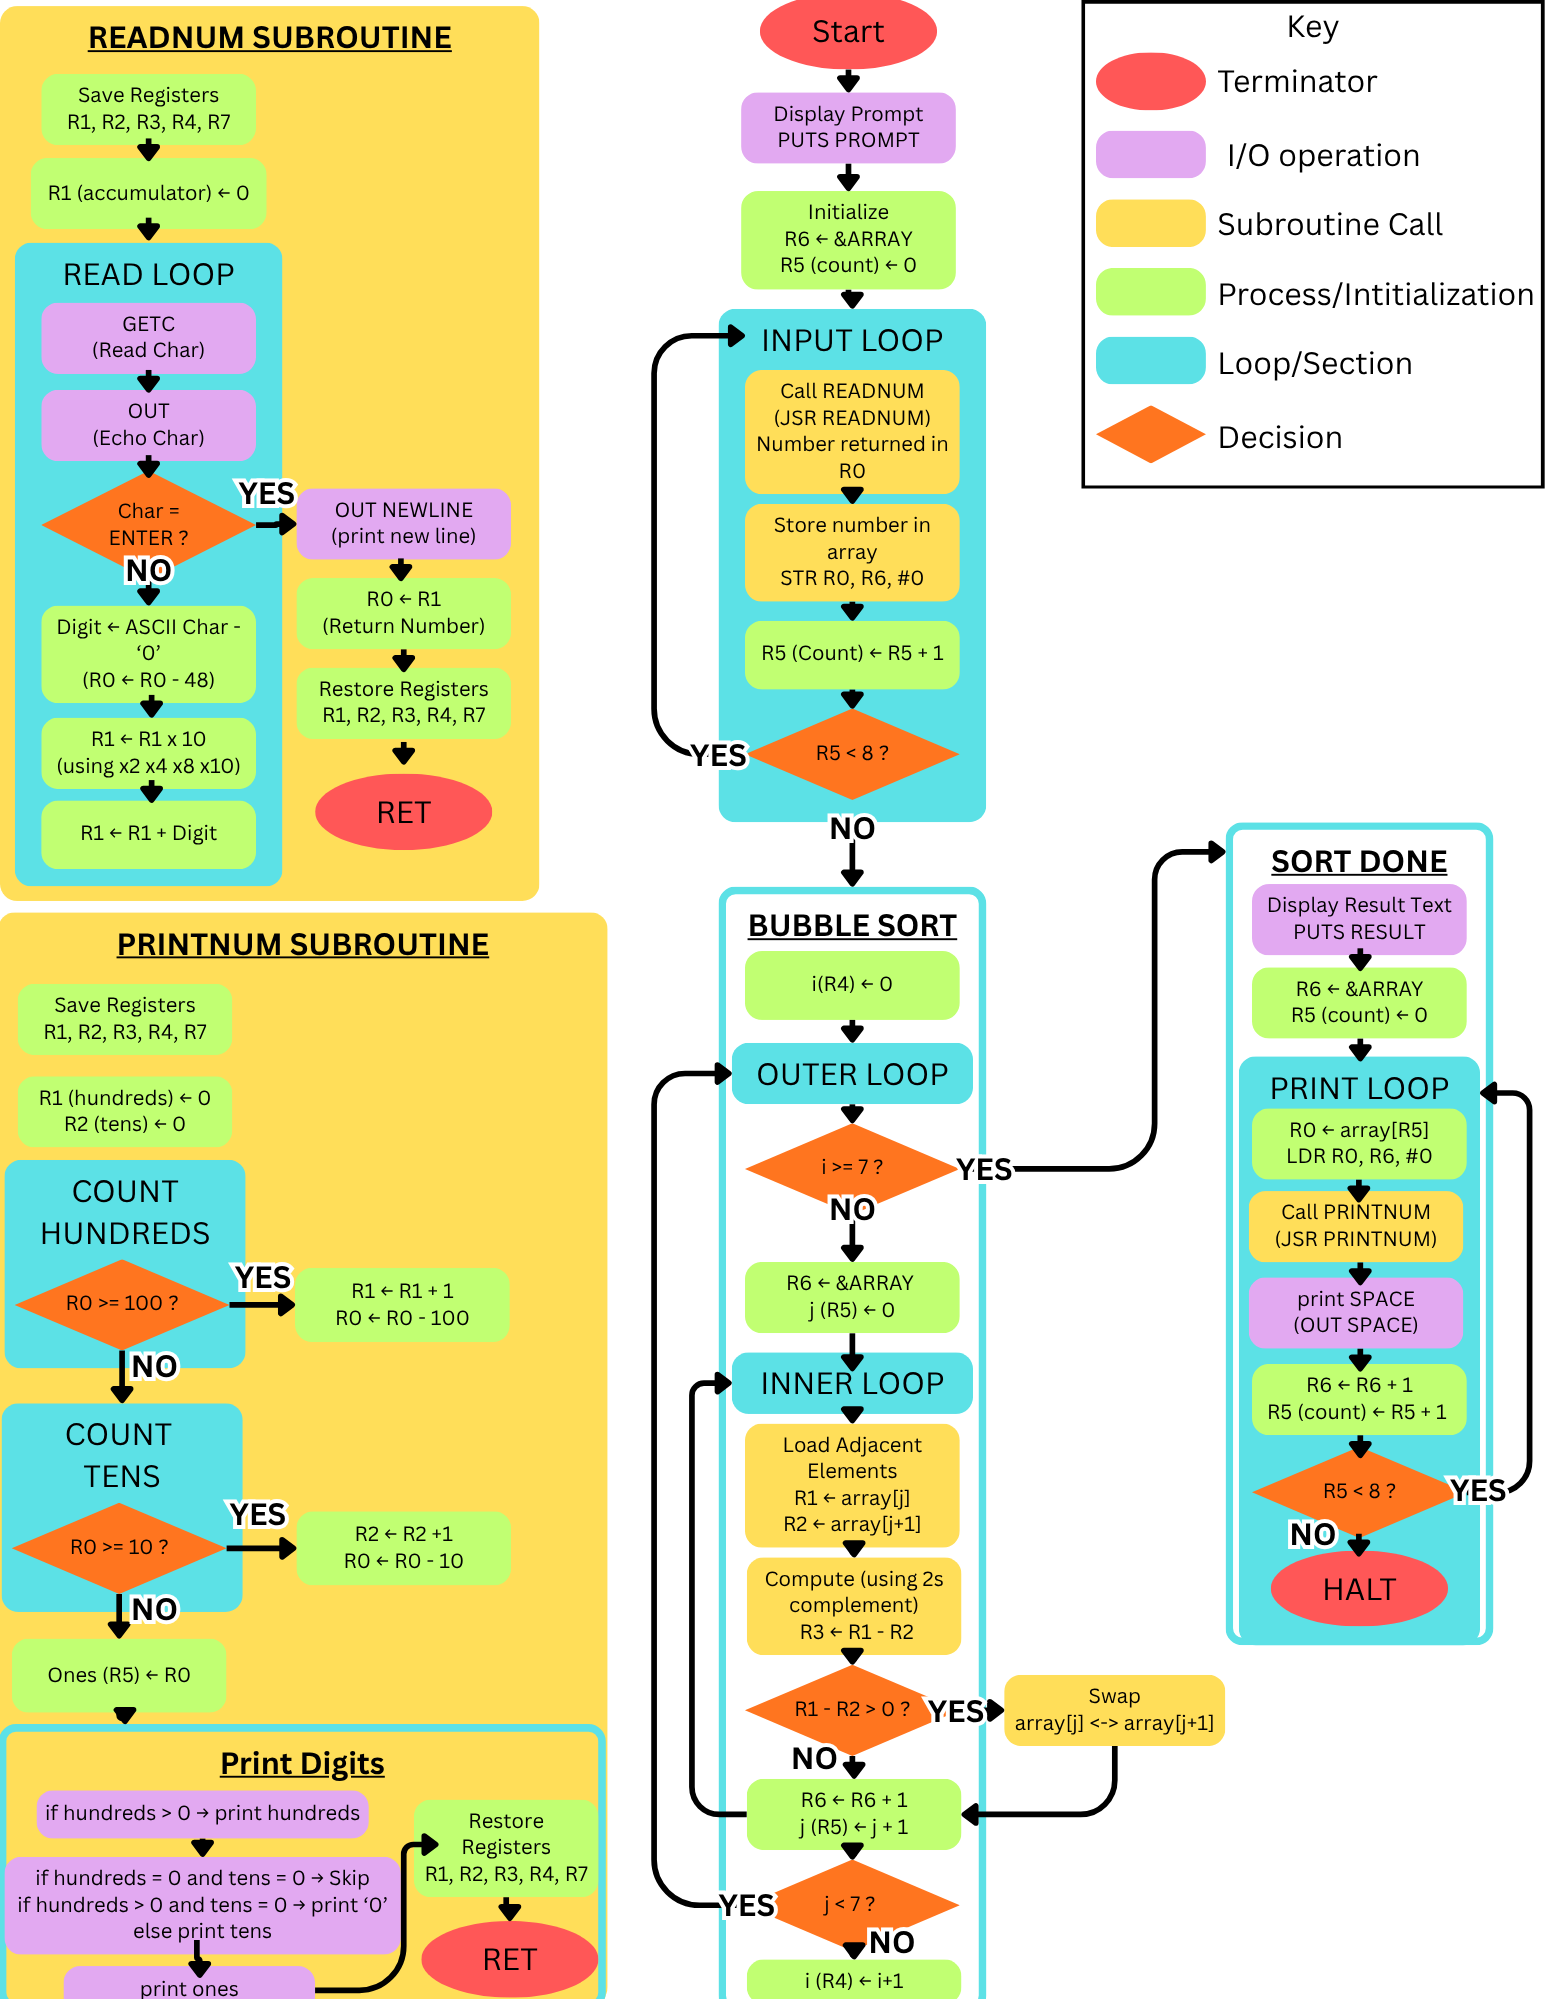
\includegraphics[width=\textwidth,keepaspectratio]{flowchart.png}
\end{center}

Symbol vocabulary, per the Key in the upper right of the figure: red oval = terminator; purple = I/O operation (PUTS, GETC, OUT); yellow = subroutine call (JSR); green = process or initialization; cyan = labelled loop or section; orange diamond = decision.


\end{document}